\newpage
\setcounter{section}{0}
\renewcommand{\thesection}{\arabic{section}}

\begin{center}
    \Huge
    \textbf{Modul 5}
    
    Implementasi dan Konfigurasi IP Version 6

\end{center}


\section{pendahuluan}

Semakin berkembangnya teknologi, maka semakin banyak alokasi alamat jaringan yang diperlukan. Maka dari itu dikembangkanlah Internet Protocol Address v6 (IPV6). Internet Protocol Address v6 (IPv6) adalah standar protokol yang digunakan untuk mengidentifikasi dan mengarahkan alamat jaringan dalam jaringan komputer. Dibandingkan dengan pendahulunya, IPv4, IPv6 memiliki format alamat yang lebih panjang dengan 128 bit, yang memungkinkan jumlah alamat yang jauh lebih besar, sehingga dapat mengatasi kekurangan alamat IPv4 yang semakin berkurang. IPv6 juga mendukung fitur-fitur tambahan, termasuk pemantauan aliran lalu lintas, keamanan yang ditingkatkan, dan kualitas layanan yang lebih baik, menjadikannya solusi jangka panjang untuk pertumbuhan Internet yang pesat dan kebutuhan alamat yang terus berkembang.

\section{Tujuan Praktikum}

\begin{enumerate}
    \item Mengetahui bagaimana konfigurasi static routing menggunakan IPV6
    \item Mengimplementasikan konfigurasi IPV6 pada perangkat mikrotik
\end{enumerate}

\section{Alat dan Bahan}

berikut adalah alat dan bahan yang digunakan:


\begin{enumerate}
    \item 2 Router
    \item 3 Kabel LAN
    \item 2 Laptop
    \item Koneksi Internet
\end{enumerate}

\section{Topologi}

berikut adalah topologi yang digunakan :

\begin{center}
    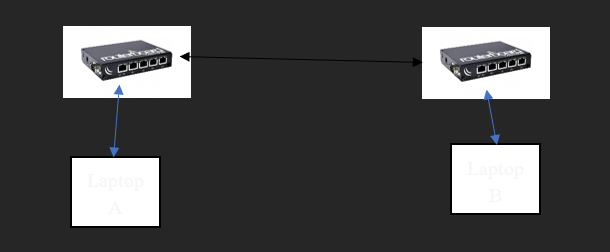
\includegraphics[width=0.7\textwidth]{image/P5/Topologi.png}    
    
    figure.1 Topologi
\end{center}


\section{Langkah Percobaan}
\begin{enumerate}
    \item 
\end{enumerate}

\section{Hasil Percobaan}


\section{Kesimpulan}


\section{Tugas modul}
